\documentclass[border=5mm]{standalone}
\usepackage{tikz}
\usetikzlibrary{calc}           % For general calculations
\usetikzlibrary{matrix}         % For the matrix cmd
\usetikzlibrary{positioning}    % For above = Xcm of and similars
\usetikzlibrary{intersections}  % Mainly here for the arc over line
\usetikzlibrary{topaths}        % Enable move to operation
\usetikzlibrary{backgrounds}    % Put colors in background
\usetikzlibrary{shapes}         % Allow use of more shapes

\tikzset{rosnode/.style={ellipse,
                        fill=blue!20,
                        matrix of nodes,
                        row sep=1mm,
                        column sep=1mm,
                        nodes={anchor=center, inner sep=0pt, outer sep=0pt}
                        },
        rostopic/.style={ellipse,
                        fill=blue!50,
                        matrix of nodes,
                        row sep=1mm,
                        column sep=1mm,
                        nodes={anchor=center, inner sep=0pt, outer sep=0pt}
        },
}

\begin{document}
\sffamily

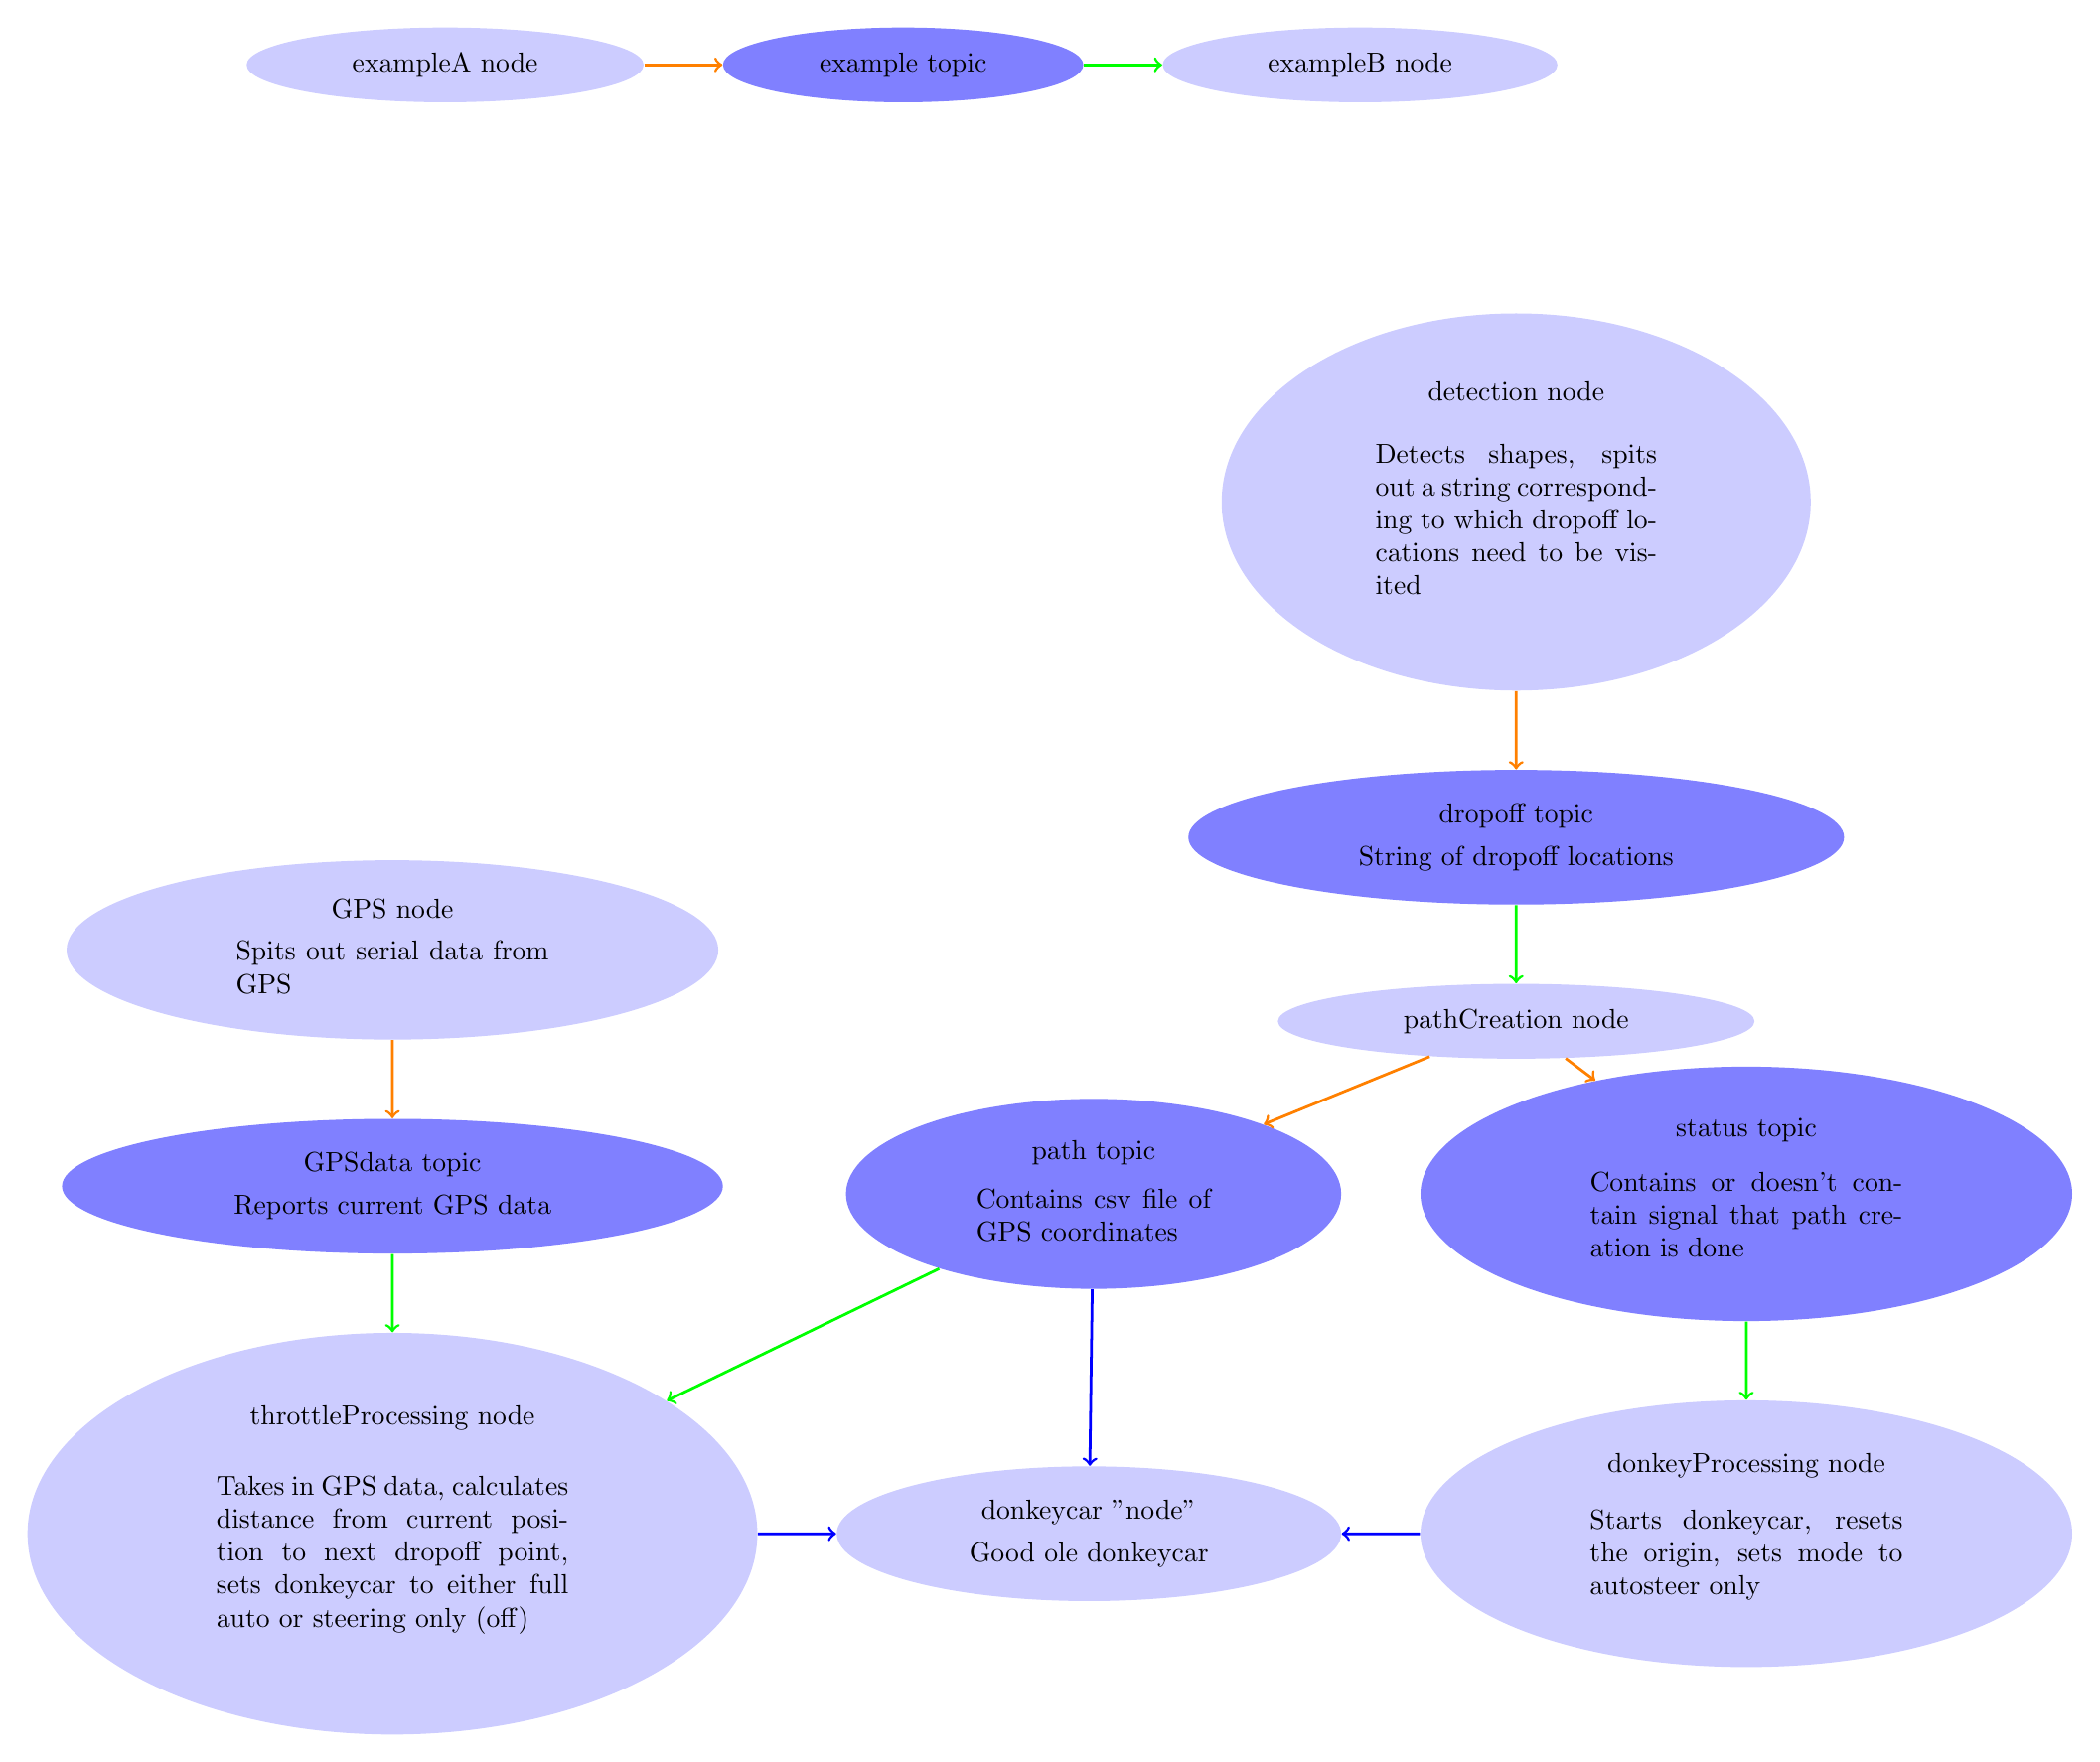
\begin{tikzpicture}
    [scale=.9,auto=center]

    % EXAMPLE
    \matrix[rosnode] (exampleA) {
        exampleA node \\
    };

    \matrix[rostopic, right= of exampleA] (exampleC) {
        example topic \\
    };

    \matrix[rosnode, right= of exampleC] (exampleB) {
        exampleB node \\
    };
    
    \draw[->,orange,line width=1pt] (exampleA) -- (exampleC);
    \draw[->,green,line width=1pt] (exampleC) -- (exampleB);


    % NODE DIAGRAM
    \matrix[rosnode, below right= 5cm of exampleC] (detection) {
        detection node \\
        \parbox{3.6cm}{Detects shapes, spits out a string corresponding to which dropoff locations need to be visited} \\
    };

    \matrix[rostopic, below= of detection] (dropoff) {
        dropoff topic \\
        String of dropoff locations \\
    };

    \matrix[rosnode, below= of dropoff] (pathCreation) {
        pathCreation node \\
    };

    \matrix[rostopic, below left= of pathCreation] (path) {
        path topic \\
        \parbox{3cm}{Contains csv file of GPS coordinates} \\
    };

    \matrix[rostopic, right= of path] (status) {
        status topic \\
        \parbox{4cm}{Contains or doesn't contain signal that path creation is done} \\
    };

    \matrix[rosnode, below= of status] (donkeyProcessing) {
        donkeyProcessing node \\
        \parbox{4cm}{Starts donkeycar, resets the origin, sets mode to autosteer only} \\
    };

    \matrix[rosnode, left= of donkeyProcessing] (donkeycar) {
        donkeycar "node" \\
        Good ole donkeycar \\
    };

    \matrix[rosnode, left= of donkeycar] (throttleProcessing) {
        throttleProcessing node \\
        \parbox{4.5cm}{Takes in GPS data, calculates distance from current position to next dropoff point, sets donkeycar to either full auto or steering only (off)} \\
    };

    \matrix[rostopic, above= of throttleProcessing] (GPSdata) {
        GPSdata topic \\
        Reports current GPS data \\
    };

    \matrix[rosnode, above= of GPSdata] (GPS) {
        GPS node \\
        \parbox{4cm}{Spits out serial data from GPS} \\
    };
    
    \draw[->,orange,line width=1pt] (detection) -- (dropoff);
    \draw[->,green,line width=1pt] (dropoff) -- (pathCreation);
    \draw[->,orange,line width=1pt] (pathCreation) -- (path);
    \draw[->,orange,line width=1pt] (pathCreation) -- (status);
    \draw[->,green,line width=1pt] (status) -- (donkeyProcessing);

    \draw[->,blue,line width=1pt] (path) -- (donkeycar);
    \draw[->,blue,line width=1pt] (donkeyProcessing) -- (donkeycar);
    \draw[->,blue,line width=1pt] (throttleProcessing) -- (donkeycar);

    \draw[->,orange,line width=1pt] (GPS) -- (GPSdata);
    \draw[->,green,line width=1pt] (GPSdata) -- (throttleProcessing);
    \draw[->,green,line width=1pt] (path) -- (throttleProcessing);
    
\end{tikzpicture}
\end{document}